The UML printed below represent an idea of how the system must be developed, in order to make it easier to be read,
we decide to insert only few example of activities and actions.
An activity is a set of object that must be shown to the users ( also the guests).
An action is something that can be activated by the user, or also by a guest, interacting with the application.
\begin{center}
\hspace*{-2cm}
 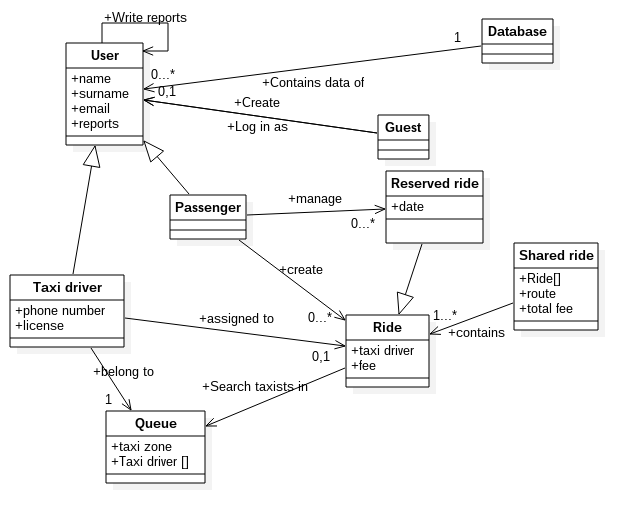
\includegraphics[height=25cm, width=18cm]{UML/RASDUML.png}
\end{center}
